\documentclass[man,12pt,floatsintext]{apa7}
\usepackage[american]{babel}
\usepackage{csquotes}
\usepackage[style=apa,sortcites=true,sorting=nyt,backend=biber]{biblatex}
\DeclareLanguageMapping{american}{american-apa}
\addbibresource{bibliography.bib}
\usepackage[T1]{fontenc}
\usepackage{mathptmx}
% --- Math/fig/table helpers (safe with apa7) ---
\usepackage{amsmath,amssymb,bm}
\usepackage{graphicx}
\usepackage{booktabs}
\usepackage{siunitx}
\usepackage{hyperref}
\usepackage{enumitem}
\usepackage{subcaption}
% for referencing sections
\usepackage{nameref}
% for table
\usepackage{threeparttable}
\usepackage{tabularx}
\usepackage{setspace}
\usepackage{array}
\usepackage{multirow}
\usepackage[table]{xcolor}
\definecolor{rulegray}{gray}{0.82}
\definecolor{bandgray}{gray}{0.97}
\newcolumntype{L}[1]{>{\raggedright\arraybackslash}m{#1}}
\newcolumntype{C}[1]{>{\centering\arraybackslash}m{#1}}
% Title page stuff _____________________
\title{When Context Looks Like Coupling: A Slow--Fast Theory of Psychological Dynamics}
\shorttitle{Slow--Fast Psychological Dynamics}
\author{%
Kyuri Park\textsuperscript{*1},
Denny Borsboom\textsuperscript{3},
Mike Lees\textsuperscript{1,2},
Lourens Waldorp\textsuperscript{3},
Johan Bollen\textsuperscript{1},
Vítor V.\ Vasconcelos\textsuperscript{1,2}
}
\affiliation{%
\textsuperscript{1} University of Amsterdam\mbox{,} Informatics Institute\mbox{,} Computational Science Lab\\
\textsuperscript{2} University of Amsterdam\mbox{,} Institute for Advanced Study\\
\textsuperscript{3} University of Amsterdam\mbox{,} Department of Psychology
}
\authornote{%
\textbf{Author contact information.}
Kyuri Park (\href{mailto:k.park@uva.nl}{k.park@uva.nl});
Vítor V.\ Vasconcelos (\href{mailto:v.v.vasconcelos@uva.nl}{v.v.vasconcelos@uva.nl});
Mike Lees (\href{mailto:m.h.lees@uva.nl}{m.h.lees@uva.nl});
Denny Borsboom (\href{mailto:d.borsboom@uva.nl}{d.borsboom@uva.nl});
Lourens Waldorp (\href{mailto:l.j.waldorp@uva.nl}{l.j.waldorp@uva.nl});
Johan Bollen (\href{mailto:j.bollen@uva.nl}{j.bollen@uva.nl}).\\[0.5em]
\textbf{Affiliation addresses.}\\
\textsuperscript{1} University of Amsterdam, Informatics Institute, Computational Science Lab,
PO Box 94323, 1090 GH Amsterdam, The Netherlands.\\
\textsuperscript{2} University of Amsterdam, Institute for Advanced Study,
Oude Turfmarkt 147, 1012 GC Amsterdam, The Netherlands.\\
\textsuperscript{3} University of Amsterdam, Department of Psychology,
Nieuwe Achtergracht 129, 1018 WS Amsterdam, The Netherlands.\\[0.5em]
\textbf{Correspondence.}
*Correspondence concerning this article should be addressed to Kyuri Park.
}
% for Psychological Review:
\abstract{
\begingroup
\setstretch{1.3}\selectfont
Many psychological states change quickly, but the conditions that shape them
often change more slowly. Symptoms, affect, attention, motivation, and behavior
can shift over short timescales, while stress exposure, social isolation,
financial strain, biological vulnerability, and environmental conditions may
persist over longer periods. This difference in timescale matters because slow
conditions can change how easily fast states become active, how long they
persist, and how easily they recover.
We develop this argument through psychopathology symptom networks. Network
models often focus on symptom--symptom coupling, but symptoms also unfold
within broader contextual conditions. We formalize this idea in a computational
slow--fast model that embeds a fast \(0/1\) symptom network within a slower
contextual field. The model separates symptom-specific activation tendencies,
symptom--symptom coupling, and slow contextual input.
We use the model in four ways. First, we show that different slow contextual
baselines can change overall symptom activation even when symptom--symptom
coupling is held fixed. Second, we show that a perturbation to the slow field
can produce temporary increases in symptom activation followed by recovery.
Third, we show that feedback from sustained symptom activation to the slow
field can slow recovery and, under stronger feedback, produce
history-dependent activation regimes. Fourth, we show that omitting the slow
field from an estimated symptom network can increase apparent connectivity.
Together, these simulations show how slow context can shape symptom activation,
recovery, persistence, history-dependence, and the interpretation of estimated
symptom networks. The results suggest that differences in estimated symptom
networks should not automatically be interpreted as differences in
symptom--symptom coupling. More broadly, the model offers a computational
framework for studying fast psychological states within slower-moving
contextual conditions.
\par
\endgroup
}
\keywords{slow--fast systems; psychological dynamics; timescale separation; symptom networks; computational modeling}
\begin{document}
\maketitle % This tells LaTeX to make the title page
%
% Revision anchor:
% This is the computational model paper extending the slow--fast perspective paper.
% The model is the contribution. The network-estimation issue is one implication.
% We present the model modularly: fast symptom network -> slow contextual field ->
% slow contextual dynamics -> stress/recovery/feedback -> estimated-network consequences.
% Scope decision:
% This is the model paper extending the slow--fast perspective paper.
% We keep the model broad enough to cover baseline slow context, stress/recovery,
% symptom-to-context feedback, and estimated-network consequences.
% The estimation problem is one implication of the model, not the whole paper.
%structure
% structure
\section{Introduction}
% Goal of revised intro:
% This is the computational model paper extending the slow--fast perspective paper.
% Start from multiscale psychological dynamics, not generic symptom-network framing.
% Then use symptom networks as the focal example.
% The model is the contribution; network-estimation consequences are one implication.
Psychological states often change faster than the conditions that shape them.
Symptoms, affect, attention, motivation, and behavior can shift over short
timescales, while stress exposure, social isolation, financial strain,
biological vulnerability, and environmental conditions often change more
slowly. These slower conditions do not simply sit outside psychological
dynamics. They can change how easily faster states become active, how long
they persist, and how easily they recover.

Psychopathology symptom networks are a useful case for this problem. Network
approaches start from the idea that symptoms do not merely co-occur; they can
influence one another \parencite{borsboom2017network, robinaugh2020network}. Insomnia may contribute to fatigue, fatigue may reduce
concentration, and concentration problems may worsen feelings of failure. In
this view, symptoms are not only indicators of an underlying disorder, but
parts of a system whose dynamics can become self-sustaining. Yet symptoms do
not unfold outside the broader conditions of a person's life. The same symptom
network may behave differently when it is embedded in different slow contextual
conditions.

This creates a problem for how estimated symptom networks are interpreted.
Researchers often compare estimated symptom networks across groups that differ
in illness course, treatment stage, or exposure history, such as persistent
versus remitted depression, admission versus discharge samples, or trauma
reporters versus non-reporters \parencite[e.g.,][]{van2015association, beard2016network, peel2021comparison}, typically
comparing global strength, specific edge weights, or centrality, often using
formal network-comparison procedures \parencite{van2023comparing, haslbeck2022estimating}.
If two groups differ in estimated network structure, the difference may be read as
a difference in symptom--symptom coupling. But a similar pattern could arise if
the groups occupy different slow contextual regimes. In that case, the estimated
network may partly reflect the conditions under which symptoms become active,
rather than a change in the coupling among symptoms themselves.

This distinction matters because the explanations point to different targets.
If group differences reflect stronger symptom--symptom coupling, intervention
may need to focus on the relations among symptoms. If they reflect slow
contextual conditions, intervention may instead need to target the conditions
that make symptoms easier to activate, harder to recover from, or more likely
to persist. The two explanations are not mutually exclusive, but they should
not be treated as the same thing.

The present paper develops a computational slow--fast model of symptom
dynamics, extending an explicitly slow--fast perspective on psychopathology
that has linked slowly evolving personality and resilience processes to
faster symptom dynamics \parencite{lunansky2020personality, <our-perspective-paper>}. The aim is not only to ask whether slow context can distort estimated
networks, but to give a model for simulating how fast symptom dynamics unfold
inside slower contextual conditions. The model embeds a fast \(0/1\) symptom
network within a slower contextual field. The fast layer represents symptom
activation and symptom--symptom coupling. The slow layer represents contextual
conditions that can shift symptom activation, recover slowly, accumulate, or be
perturbed by stressors.

We use the model in four steps. First, we ask whether different slow contextual
baselines can change overall symptom activation even when symptom--symptom
coupling is held fixed. Second, we ask how a perturbation to the slow field
shapes stress and recovery. Third, we ask how symptom-to-context feedback
changes recovery, and whether stronger feedback can produce history-dependent
activation regimes. Fourth, we ask what an estimated symptom network recovers
when the slow field is omitted from the statistical model.

These simulations are not four separate arguments. They are four uses of the
same model. Together, they show how slow context can shape symptom activation, recovery,
persistence, history-dependence, and the interpretation of estimated symptom networks.
Our goal is not to replace symptom-network theory with a contextual account.
Rather, we formalize a way to put the two in the same model. This allows us to
separate three quantities that are often difficult to disentangle in empirical
network comparisons: symptom-specific activation tendencies, symptom--symptom
coupling, and slow contextual input.

\section{A slow--fast model of symptom dynamics}
% Goal:
% Present the model in modules, not all at once.
% Denny's model comments are handled here.
% We use an uncentered 0/1 symptom-network model with symptom-specific thresholds.
\subsection{Fast symptom network}
% Introduce S_i in {0,1}.
% Introduce tau_i and omega_ij.
% No slow context yet.
We first define the fast layer of the model. Let \(S_i\in\{0,1\}\)
denote whether symptom \(i\) is inactive or active. The fast layer follows a
\(0/1\) symptom-network formulation \parencite{van2014new, marsman2018introduction} in which the activation probability of each
symptom depends on its own baseline activation tendency and on the current
state of the other symptoms:
\[
\operatorname{logit}\Pr(S_i^{\mathrm{new}}=1\mid \mathbf S_{-i})
=
\tau_i+\sum_{j\neq i}\omega_{ij}S_j .
\]
Here, \(\tau_i\) is the baseline activation tendency of symptom \(i\), and
\(\omega_{ij}\) is the coupling from symptom \(j\) to symptom \(i\). In this
parameterization, \(\tau_i\) has a direct interpretation: it is the activation
tendency of symptom \(i\) when the other symptoms are inactive. Active symptoms
then add to this tendency through the couplings \(\omega_{ij}\).

In the simulations, one fast step consists of a random-order sweep through the
symptoms, updating each symptom once conditional on the current states of the
others. We write \(S_i^{\mathrm{new}}\) to emphasize that the update is local to
the symptom being updated, rather than a synchronous update of all symptoms at
once.

This choice is important for the present argument. We want to keep the
interpretation of symptom-specific activation tendencies separate from the
interpretation of symptom--symptom coupling. For this reason, the revised model
uses the uncentered \(0/1\) formulation above rather than a centered mean-field
term such as \(J(m-\frac{1}{2})\). A centered term can be useful for some
statistical-physics purposes, but in the present setting it makes the baseline
activation tendency depend on the coupling parameter. The uncentered
formulation keeps the pieces of the model closer to their psychological
interpretation: symptoms can have different baseline tendencies, and active
symptoms can increase the activation tendency of other symptoms.

\subsection{Adding a slow contextual field}
% Add P_t.
% Explain P_t as slow context, not another fast symptom.
% Explain gamma_i as symptom-specific sensitivity to context.
The slow--fast extension adds a contextual field \(P_t\) that changes more
slowly than the symptoms themselves:
\[
\operatorname{logit}\Pr(S_i^{\mathrm{new}}=1\mid \mathbf S_{-i},P_t)
=
\tau_i+\sum_{j\neq i}\omega_{ij}S_j+\gamma_iP_t .
\]
The slow field \(P_t\) represents contextual conditions that are not symptoms
but can change how easily symptoms become active. Examples include chronic
stress, social isolation, financial strain, biological vulnerability, and
persistent environmental adversity. The loading \(\gamma_i\) allows symptoms to
differ in how strongly they respond to this field.

This formulation separates three quantities. The first is the symptom-specific
activation tendency, \(\tau_i\). The second is symptom--symptom coupling,
\(\omega_{ij}\). The third is slow contextual input, \(\gamma_iP_t\). The model
therefore allows the same symptom network, with the same coupling matrix
\(\omega\), to behave differently when it is embedded in a different slow
contextual field.

\subsection{Slow contextual dynamics}
% Introduce slow movement of P_t only after the fast layer is clear.
% Keep it simple in the main text.
% Details/noise/shocks can go to appendix if needed.
The slow field can be treated in two ways. In the simplest case, \(P_t\) is a
stable contextual condition that differs across people or groups. For example,
one group may have a higher contextual baseline than another group:
\[
P_t = P_{\mathrm{base}}^{(g)} .
\]
This simple case is useful because it isolates the main point: the same fast
symptom network can behave differently when it is observed under different
slow contextual conditions.

In the fuller slow--fast model, \(P_t\) is allowed to change over time. We
model this as a slow process that tends to return toward a contextual baseline,
but can also fluctuate, be perturbed by stressors, or be affected by sustained
symptom activation:
\[
P_{t+\Delta t}
=
P_t
+
\kappa(P_{\mathrm{base}}-P_t)\Delta t
+
\sigma_P\sqrt{\Delta t}\epsilon_t
+
\xi_t
+
b[\bar m_t-m^\star]_+\Delta t .
\]
Here, \(\kappa\) controls how quickly the slow field returns toward its
baseline \(P_{\mathrm{base}}\). The term
\(\sigma_P\sqrt{\Delta t}\epsilon_t\) represents small background fluctuations
in the slow field. The jump term \(\xi_t\) represents occasional larger
perturbations, such as acute stressors \parencite{cohen2019ten, dohrenwend2006inventorying}. The final term allows sustained symptom
activation above a reference level to feed back into the slow field. We use the
positive part \([\bar m_t-m^\star]_+\) so that this feedback represents
symptom-related deterioration rather than treating low symptom activation as an
additional protective force.

This term is meant to capture feedback from sustained symptom activation, not an immediate effect of a single symptom at a single time point. The smoothed quantity \(\bar m_t\) summarizes recent mean symptom activation, and
\(m^\star\) is a reference activation level. In the simulations below, we turn this term off when we want to isolate the effect of slow context on symptoms,
and turn it on when we ask how symptoms may feed back into the slow field, in line with stress-generation accounts in which sustained distress increases exposure to later adversity \parencite{hammen2006stress, liu2010stress, rnic2023vicious}.

\begin{figure}[htbp]
  \centering
  
\includegraphics[width=\linewidth]{figs/revision_2026/slow-fast-model-illustration_v2.png}
  \caption{\textbf{Conceptual schematic of the slow--fast symptom model.}
  The fast layer consists of binary symptoms that activate and deactivate on a
  short timescale. Symptoms can influence one another through the coupling
  matrix \(\omega\). The slow layer is represented by a contextual field
  \(P_t\), which changes more gradually and shifts symptom activation through
  the input \(\gamma_iP_t\). The model also allows feedback from the fast layer
  to the slow layer: sustained mean symptom activation, summarized by
  \(\bar m_t\), can push the slow field upward through
  \(b[\bar m_t-m^\star]_+\). Acute perturbations enter the slow field through
  \(\xi_t\). Thus, the same symptom network can behave differently depending
  on the slower contextual conditions in which it is embedded.}
  \label{fig:slow-fast-illust}
\end{figure}

Figure~\ref{fig:slow-fast-illust} provides a schematic overview of this coupling between the fast and slow layers.

We introduce these components separately in the simulations below. The first
simulations use the simpler case in which slow context differs across people or
groups but the symptom--symptom coupling matrix is held fixed. Later simulations
add stressor perturbations and symptom-to-context feedback. This staged approach
keeps the roles of slow baseline, slow fluctuation, acute perturbation, and
feedback separate.

\subsection{What the model lets us ask}
% The model is the tool.
% It lets us simulate:
% 1. different slow-context baselines
% 2. stress and recovery
% 3. feedback and persistence
% 4. what estimated networks recover when slow context is omitted
The model is meant to be a tool for thinking through slow--fast psychological
dynamics. It lets us ask what changes when a fast symptom network is embedded
in a slower contextual process. In particular, we use it to examine four
questions.

First, can groups show different symptom activation level even when their
symptom--symptom coupling is the same? Second, how does a slow contextual field
shape recovery after a stressor? Third, can feedback from sustained symptoms to
the slow field make symptom activation more persistent? Fourth, what does an
estimated symptom network recover when the slow contextual field is omitted
from the statistical model?

These questions are connected by the same basic issue: estimated symptom
dynamics may reflect both fast coupling among symptoms and slower conditions
that change the ease with which symptoms become active.

Throughout the simulations, we summarize the fast symptom state in two ways.
Let
\[
M_t=\sum_{i=1}^{N}S_{i,t}
\]
denote the number of active symptoms, and let
\[
m_t=\frac{1}{N}\sum_{i=1}^{N}S_{i,t}
\]
denote mean symptom activation, or the fraction of symptoms active. These
quantities summarize the state of the symptom layer; they do not replace the
symptom-level dynamics, which are simulated at the level of individual binary
symptoms.

\section{Simulation overview}
The simulations use the model as a controlled theoretical tool. They are not
intended to calibrate a specific clinical population. Instead, they ask what
kinds of patterns can arise when fast symptom dynamics are embedded in a slower
contextual field. Across simulations, the symptom--symptom coupling matrix is
held fixed. What changes is the slow contextual condition, the dynamics of the
slow field, the presence or absence of symptom-to-context feedback, or whether
the slow field is included in the statistical model.

We organize the simulations in four steps. Simulation 1 isolates the effect of
slow contextual baseline: the same fast symptom network is observed under low,
middle, and high values of the slow field. Simulation 2 introduces an acute
perturbation to the slow field and asks how symptoms respond as the slow field
recovers. Simulation 3 adds symptom-to-context feedback and asks whether
feedback slows recovery under moderate feedback and produces history-dependent
activation regimes under stronger feedback. Simulation 4 turns to the
observation problem and asks what an estimated symptom network recovers when
data are generated by the slow--fast model but the slow field is omitted from
the statistical model.

This order follows the logic of the model. We first show that slow context can
shift overall symptom activation without changing coupling. We then allow the
slow context to move and recover. We then allow symptoms to feed back into that
slow field, first as a recovery delay and then as a possible source of
history-dependence. Finally, we ask how the same slow--fast process appears to
a researcher who estimates a symptom-only network.

\subsection{Simulation 1: Slow context shifts symptom activation under fixed coupling}
% Same tau_i, omega_ij, gamma_i across groups.
% Different slow contextual baseline or P_t.
% Question: can symptom burden differ without coupling differences?
The first simulation isolates the effect of slow contextual baseline. We use
the same fast symptom network in all conditions, with the same thresholds
\(\tau_i\), couplings \(\omega_{ij}\), and context sensitivities \(\gamma_i\).
Only the slow contextual baseline differs. This asks whether the same symptom
system can produce different levels of overall activation simply because it is
embedded in a different slow context.

This simulation is the simplest demonstration of the model. If two groups
differ in symptom activation here, the difference cannot be attributed to
different symptom--symptom coupling, because the coupling matrix is fixed by
design.

\paragraph{Design.}
Simulation 1 used a fixed fast symptom network and varied only the slow
contextual baseline (Table~\ref{tab:sim1_parameters}). The fast layer contained \(N=9\) binary symptoms, chosen
to match the size of a typical PHQ-9 symptom network \parencite{cramer2016major}. The same threshold vector
\(\tau\), coupling matrix \(\omega\), and context-loading vector \(\gamma\)
were used in all conditions. The only difference between conditions was the
value of the slow contextual field \(P\).

We used three contextual baselines:
\[
P \in \{-0.6, 0, 0.6\},
\]
which we refer to as low, middle, and high slow-context conditions. These
values are not intended as calibrated clinical quantities. They are theoretical
settings used to show how the same fast symptom network behaves under different
slow contextual fields.

The fast symptom network followed
\[
\operatorname{logit}\Pr(S_i^{\mathrm{new}}=1\mid \mathbf S_{-i},P)
=
\tau_i+\sum_{j\neq i}\omega_{ij}S_j+\gamma_iP .
\]
For each condition, we simulated repeated trajectories from the same network.
At each fast step, symptoms were updated conditionally on the current state of
the other symptoms and the fixed value of \(P\). We discarded an initial burn-in
period and summarized the post-burn-in symptom states.

\paragraph{Quantities of interest.}
Because \(\omega\) was fixed across all conditions, any difference in the
number of active symptoms or in mean symptom activation across conditions was
generated by the slow contextual field, not by a difference in
symptom--symptom coupling.

\begin{table}[ht]
\centering
\caption{Simulation 1 parameters.}
\label{tab:sim1_parameters}
\begin{tabular}{lll}
\hline
Parameter & Meaning & Value in Simulation 1 \\
\hline
\(N\) & Number of symptoms & 9 \\
\(\tau_i\) & Symptom-specific baseline activation tendency & Heterogeneous fixed vector \\
\(\omega_{ij}\) & Symptom--symptom coupling & Fixed sparse positive matrix \\
\(\gamma_i\) & Sensitivity to slow context & Heterogeneous fixed vector \\
\(P\) & Slow contextual field & \(-0.6, 0, 0.6\) \\
\(T_{\mathrm{burn}}\) & Burn-in period & 200 sweeps \\
\(T_{\mathrm{post}}\) & Post-burn-in samples & 200 sweeps per chain \\
Chains & Independent trajectories per condition & 200 \\
\hline
\end{tabular}
\end{table}

\paragraph{Results.}
Changing the slow contextual field shifted overall symptom activation even
though the symptom--symptom coupling matrix was identical across conditions. In
the low-context condition (\(P=-0.6\)), the mean number of active symptoms was
\(M=1.64\), or \(m=0.18\) of symptoms active. In the middle-context condition
(\(P=0\)), the mean number of active symptoms increased to \(M=2.49\)
(\(m=0.28\)). In the high-context condition (\(P=0.6\)), it increased further
to \(M=3.56\) (\(m=0.40\); Figure~\ref{fig:context-baseline}A).

The probability of five or more active symptoms showed the same pattern. This
probability was \(0.017\) in the low-context condition, \(0.084\) in the
middle-context condition, and \(0.268\) in the high-context condition (Figure~\ref{fig:context-baseline}B). Thus,
the same fast symptom network produced different activation distributions when
embedded in different slow contextual fields.

\begin{figure}[ht]
\centering
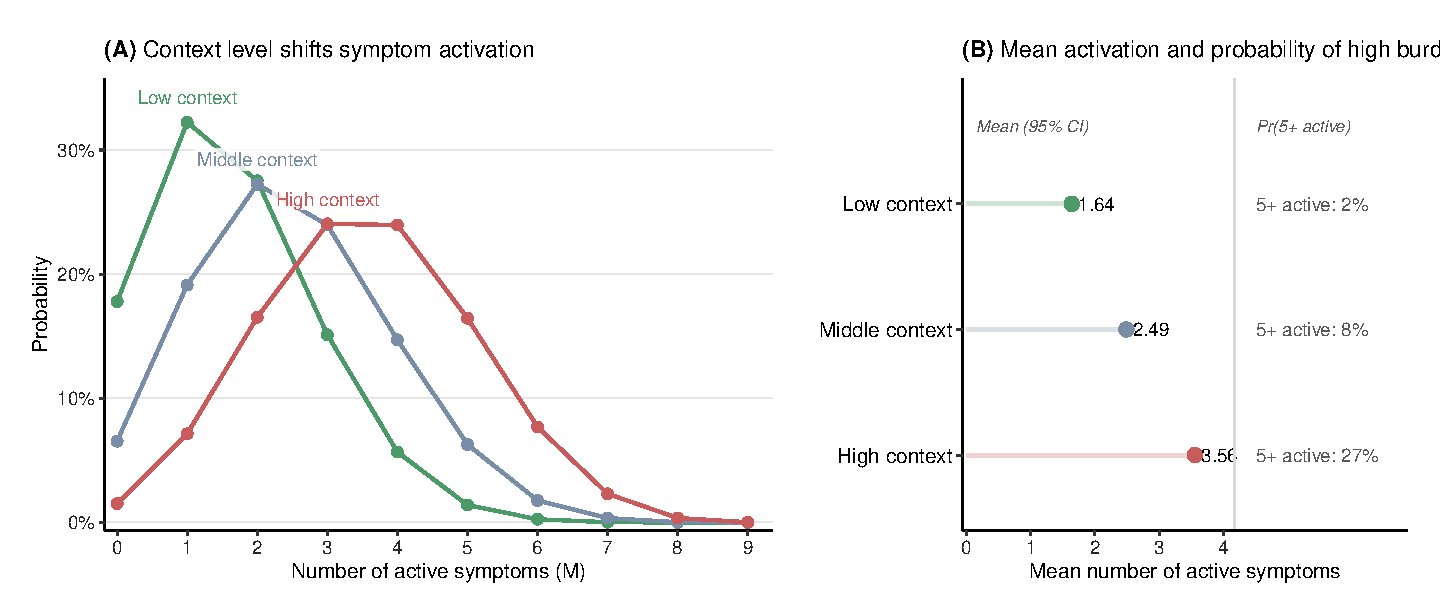
\includegraphics[width=\textwidth]{figs/revision_2026/Figure2_context_baseline.pdf}
\caption{\textbf{Slow contextual level shifts overall symptom activation under fixed symptom coupling.}
(A) The distribution of the number of active symptoms shifts toward higher activation as the slow contextual level \(P\) increases.
(B) Mean number of active symptoms and the probability of five or more active symptoms both increase across slow-context conditions.}
\label{fig:context-baseline}
\end{figure}

\subsection{Simulation 2: Stress and recovery in a slow contextual field}
% Acute perturbation to P_t.
% Show temporary recovery vs persistent elevation depending on slow parameters.
The second simulation introduces an acute perturbation to the slow contextual
field. The perturbation does not directly turn symptoms on. Instead, it changes
the slow field \(P_t\), which then shifts the activation tendency of symptoms
through the term \(\gamma_iP_t\). This allows us to examine how recovery in the
slow layer shapes recovery in the fast symptom layer.

The point of this simulation is to separate an immediate symptom fluctuation
from a slower change in the conditions under which symptoms become likely. A
short-lived perturbation can produce different symptom trajectories depending
on how quickly the slow field returns to baseline and on where the system was
before the perturbation occurred.

\paragraph{Design.}
Simulation 2 used the same fast symptom network as Simulation 1, but allowed
the slow contextual field \(P_t\) to change over time (Table~\ref{tab:sim2_parameters}). The slow field followed
mean-reverting dynamics with small background fluctuations:
\[
P_{t+\Delta t}
=
P_t+\kappa(P_{\mathrm{base}}-P_t)\Delta t
+\sigma_P\sqrt{\Delta t}\epsilon_t+\xi_t .
\]
Feedback from symptoms to the slow field was turned off in this simulation
(\(b=0\)). This allows the effect of an acute perturbation to the slow field to
be examined without symptom-to-context feedback.

We initialized the slow field at \(P_{\mathrm{base}}=0\). After a burn-in
period, we introduced a single positive perturbation of size \(\xi_t=1\). The
fast symptom network was updated at each step conditional on the current value
of \(P_t\). Thus, the perturbation did not directly activate symptoms. It first
changed the slow field, which then shifted symptom activation through the term
\(\gamma_iP_t\).

\begin{table}[ht]
\centering
\caption{Simulation 2 parameters.}
\label{tab:sim2_parameters}
\begin{tabular}{lll}
\hline
Parameter & Meaning & Value in Simulation 2 \\
\hline
\(N\) & Number of symptoms & 9 \\
\(\tau_i\) & Symptom-specific baseline activation tendency & Same as Simulation 1 \\
\(\omega_{ij}\) & Symptom--symptom coupling & Same as Simulation 1 \\
\(\gamma_i\) & Sensitivity to slow context & Same as Simulation 1 \\
\(P_{\mathrm{base}}\) & Slow-context baseline & 0 \\
\(\kappa\) & Mean-reversion rate & 0.20 \\
\(\sigma_P\) & Slow-field diffusion scale & 0.04 \\
\(\Delta t\) & Slow time step & 0.02 \\
\(\xi_t\) & Acute perturbation & 1.00 at shock onset \\
\(b\) & Symptom-to-context feedback & 0 \\
Burn-in & Pre-shock burn-in & 200 steps \\
Post-shock window & Recovery period & 750 steps \\
Chains & Independent trajectories & 200 \\
\hline
\end{tabular}
\end{table}

\paragraph{Results.}
Before the perturbation, the slow field remained near its baseline
(\(P\approx 0.00\)), and the mean number of active symptoms was about
\(M=2.48\) out of 9. At shock onset, the slow field increased to approximately
\(P=1.00\). Symptom activation rose shortly afterward, reaching a peak of about
\(M=4.73\) active symptoms.

By the end of the recovery window, the slow field had returned close to
baseline (\(P\approx 0.06\)), and symptom activation had also largely recovered
(\(M\approx 2.58\)). Thus, an acute perturbation to the slow field produced a
temporary increase in symptom activation without changing the symptom--symptom
coupling matrix. In this simulation, persistence was limited because feedback
from symptoms to the slow field was turned off.

\subsection{Simulation 3: Feedback, recovery, and history-dependence}
The third simulation adds feedback from sustained symptom activation to the
slow contextual field. In the previous simulation, the slow field affected
symptoms, but symptoms did not affect the slow field. Here, symptom activation
can also shift the slow field itself. This captures a simple idea: symptoms may
become more persistent when they start to change the conditions that maintain
them. For example, sustained fatigue, withdrawal, or concentration problems may
worsen work, social, or daily functioning, which in turn may make later symptom
activation more likely, consistent with stress-generation accounts of psychopathology \parencite{hammen2006stress, liu2010stress, rnic2023vicious}.

This simulation asks two related questions. First, under the moderate feedback
value used in the main recovery comparison, does symptom-to-context feedback
make recovery slower after a perturbation? Second, when feedback is stronger,
can the same slow--fast architecture produce history-dependent activation
regimes, in which late symptom activation depends on the system's earlier
state, echoing critical-transition accounts of psychopathology \parencite{van2014critical, scheffer2009early, helmich2021early}?

\paragraph{Design.}
Simulation 3 used the same stress-and-recovery design as Simulation 2, but
added symptom-to-context feedback. The moderate-feedback comparison used
\(b=0.50\), a value that produced a visible delay in recovery while trajectories
continued to decay toward baseline. All other parameters were kept the same as
in Simulation 2, including the fast symptom network, the shock magnitude, the
mean-reversion rate, the diffusion scale, and the time step.

Feedback was implemented as
\[
b[\bar m_t-m^\star]_+\Delta t,
\]
where \([x]_+=\max(x,0)\). The smoothed symptom signal \(\bar m_t\) was updated
with an exponential moving average, and \(m^\star\) was set to the mean symptom
activation in the \(P=0\) condition from Simulation 1. Thus, only sustained
symptom activation above the reference level contributed to an upward shift in
the slow field. Below-reference symptom activation was not treated as an
additional protective force.

To ask whether slowed recovery is simply a matter of degree or reflects a
different dynamical regime, we repeated the same shock across a wider range of
feedback strengths, holding every other parameter fixed. We also ran an
independent history-dependence check: for each feedback strength, we compared
long trajectories started from a low-activation state with trajectories started
from a high-activation state, without applying a shock. We summarized
history-dependence by the difference in late mean symptom activation between
these two initial conditions. Values near zero indicate reconvergence; larger
positive values indicate that late activation remains dependent on the initial
state.

\paragraph{Results.}
Before the shock, both conditions were close to baseline. With feedback off,
the mean slow field during the last 50 pre-shock steps was approximately
\(P=-0.003\), and the mean number of active symptoms was \(M=2.50\). With
feedback on (\(b=0.50\)), the corresponding values were \(P=0.013\) and
\(M=2.52\).

The immediate post-shock response was similar across conditions, as expected.
In the first 20 post-shock steps, peak activation was \(M=4.34\) active
symptoms with feedback off and \(M=4.43\) with feedback on. The difference
emerged during recovery. By the end of the recovery window, the slow field had
nearly returned to baseline when feedback was off (\(P=0.05\)), but remained
higher when feedback was on (\(P=0.24\)). Symptom activation showed the same
pattern, returning to \(M=2.57\) with feedback off but remaining higher with
feedback on (\(M=2.89\); Figure~\ref{fig:recovery-feedback}A).

The broader feedback sweep showed that recovery slowed as \(b\) increased. At
the moderate value used in the main recovery comparison (\(b=0.50\)), the
system remained in a convergent regime. At stronger feedback values, especially around \(b=1.0\), mean symptom
activation remained elevated within the simulated window rather than returning toward the pre-shock level (Figure~\ref{fig:recovery-feedback}B).

The history-dependence check showed that this was not only slower recovery.
In this parameter grid, history-dependence emerged around \(b\approx1.0\):
trajectories initialized from low versus high activation states no longer
converged to the same late state. The feedback strength used in the main
recovery comparison (\(b=0.50\)) falls within the convergent regime, so
history-dependence is a regime the model can exhibit under stronger feedback,
not an assumption built into the main results (Figure~\ref{fig:recovery-feedback}C).

\begin{figure}[htbp]
\centering
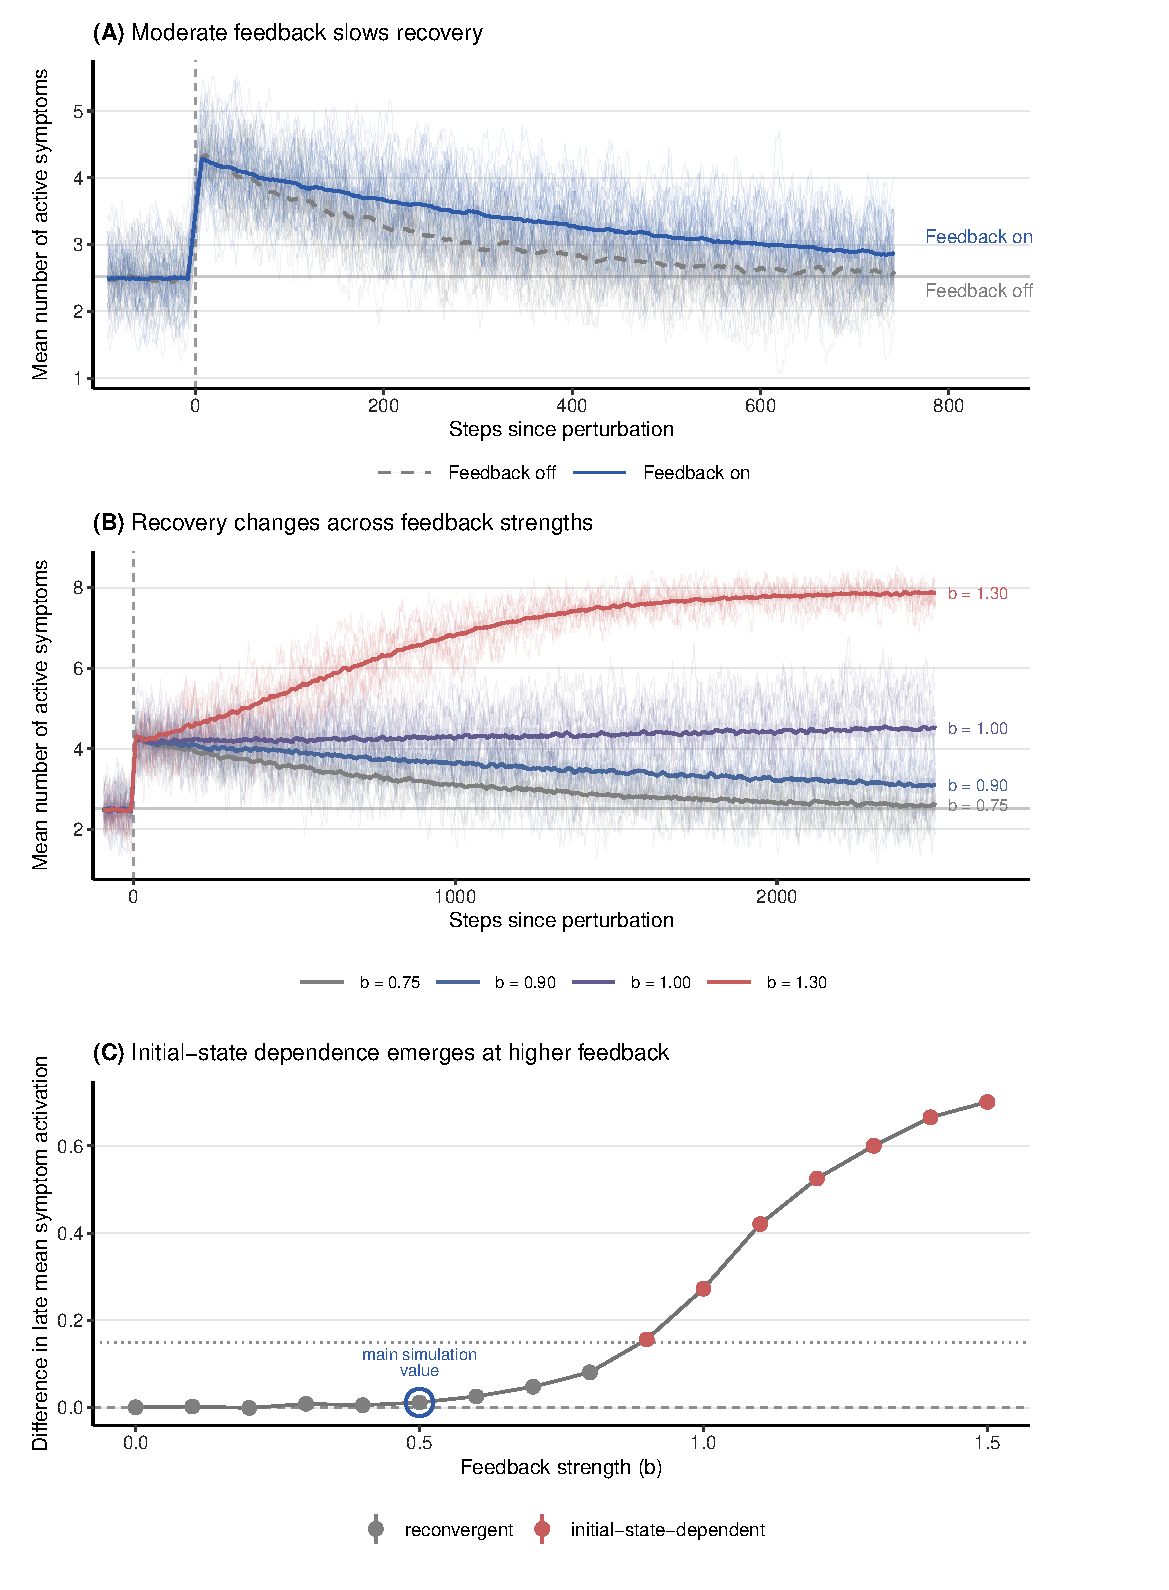
\includegraphics[width=\textwidth]{figs/revision_2026/Figure3_regimes.pdf}
\caption{\textbf{Feedback strength governs recovery and history-dependence in the slow--fast model.}
(A) Under the moderate-feedback level used in the main recovery comparison (\(b=0.50\)), an acute perturbation is followed by a transient rise in mean symptom activation. Feedback prolongs activation relative to the feedback-off condition, but both trajectories remain in the convergent regime.
(B) Applying the same perturbation across stronger feedback values shows progressively slower recovery and, at higher feedback strengths, sustained elevation within the simulated window.
(C) A history-dependence index summarizes whether late mean symptom activation depends on the system's initial state. Values near zero indicate reconvergence; larger values indicate that trajectories initialized from low versus high activation states remain separated. The main simulation value (\(b=0.50\)) falls within the convergent regime.}
\label{fig:recovery-feedback}
\end{figure}

\subsection{Simulation 4: What estimated networks recover}
The final simulation turns from the data-generating model to the observation
problem. The previous simulations used the slow--fast model to generate symptom
trajectories. Here we ask what happens when data generated by the same model
are analyzed with a symptom-only network model that omits the slow contextual
field.

This simulation is not meant to show that estimated symptom networks are
unusable or that all estimated edges are artifacts. Instead, it asks whether
unmodeled slow context can be absorbed into apparent symptom--symptom coupling,
a dynamic instance of the more general equivalence between direct interaction,
common-cause, and latent-variable representations of symptom associations
\parencite{kruis2016three, marsman2018introduction, van2021latent}. That is the estimation implication of the slow--fast model.

\paragraph{Design.}
We generated cross-sectional symptom profiles from the revised \(0/1\)
symptom-network model. Each simulated person had one observed symptom profile.
The fast symptom network, thresholds, and context loadings were the same as in
the previous simulations. The true coupling matrix \(\omega\) was therefore
fixed and known.

We compared three arms. In the fixed-context baseline arm, all simulated people
had the same contextual value, \(P=0\). In the pooled symptom-only arm, each
person had a contextual value drawn from
\[
P_i \sim \mathrm{Uniform}(-0.6,0.6),
\]
but the estimated network did not include \(P_i\). In the pooled
context-adjusted arm, the same pooled data were analyzed again, but \(P_i\) was
included as a covariate in the nodewise regressions. Thus, the symptom-only and
context-adjusted arms used the same observations; they differed only in whether
the slow contextual field was modeled.

For each arm, networks were estimated with nodewise logistic regressions
\parencite{ravikumar2010high, mukherjee2024logistic} and
then symmetrized. We repeated the full procedure across 30 independent
replicates, with 3000 simulated people per arm in each replicate. We compared estimated global strength, mean absolute edge-estimation error
relative to the true coupling matrix, and the number of apparent edges above 0.10 among symptom pairs with no true direct coupling.

\paragraph{Results.}
The symptom-only model that omitted the slow field estimated stronger apparent
connectivity than the context-adjusted model. Across 30 replicates, mean
estimated global strength was highest in the pooled symptom-only arm
(6.45, \(SE=0.08\)), lower in the fixed-context baseline arm
(5.46, \(SE=0.10\)), and lower still in the context-adjusted arm
(5.26, \(SE=0.08\)). The same pattern appeared in edge-estimation error. Mean
absolute edge-estimation error across all edges was \(0.104\) in the
symptom-only arm, \(0.090\) in the fixed-context baseline arm, and \(0.086\) in
the context-adjusted arm.

The difference was especially clear among symptom pairs with no true direct
coupling. Mean absolute edge-estimation error for truly absent edges was
\(0.106\) in the symptom-only arm and \(0.087\) in the context-adjusted arm.
The symptom-only model also produced more apparent edges above 0.10 among
truly uncoupled pairs (11.83, \(SE=0.42\)) than the context-adjusted model
(8.70, \(SE=0.37\); Figure~\ref{fig:network-estimation}B--C).

The paired replicate comparisons confirmed that this was a consistent effect.
In all 30 replicates, the symptom-only model estimated higher global strength
than the context-adjusted model. It also had higher edge-estimation error among
truly absent edges in all 30 replicates. On average, omitting the slow field
increased estimated global strength by \(1.19\) (\(SE=0.05\)) and increased
mean absolute edge-estimation error among truly absent edges by \(0.019\)
(\(SE=0.001\); Figure~\ref{fig:network-estimation}D--E).

Thus, when symptom profiles were pooled across different slow-context values,
omitting the slow field made the estimated network look more strongly connected
than the context-adjusted network. This does not mean that estimated edges are
always spurious. It shows that apparent symptom--symptom coupling can partly
reflect unmodeled slow contextual variation.

\begin{figure}[ht]
\centering
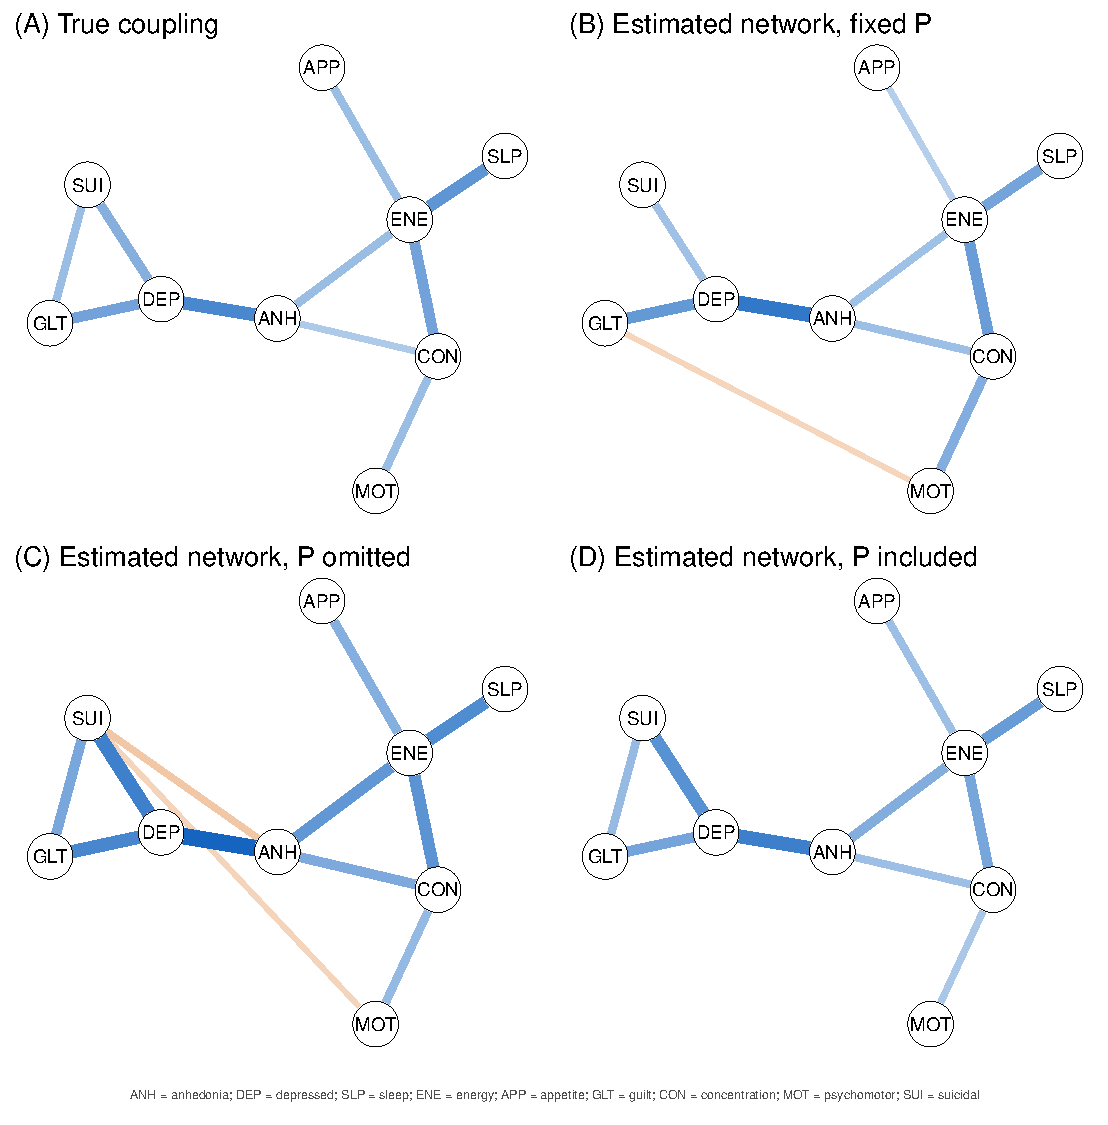
\includegraphics[width=\textwidth]{figs/revision_2026/Figure4_network_trio.pdf}
\vspace{0.75em}
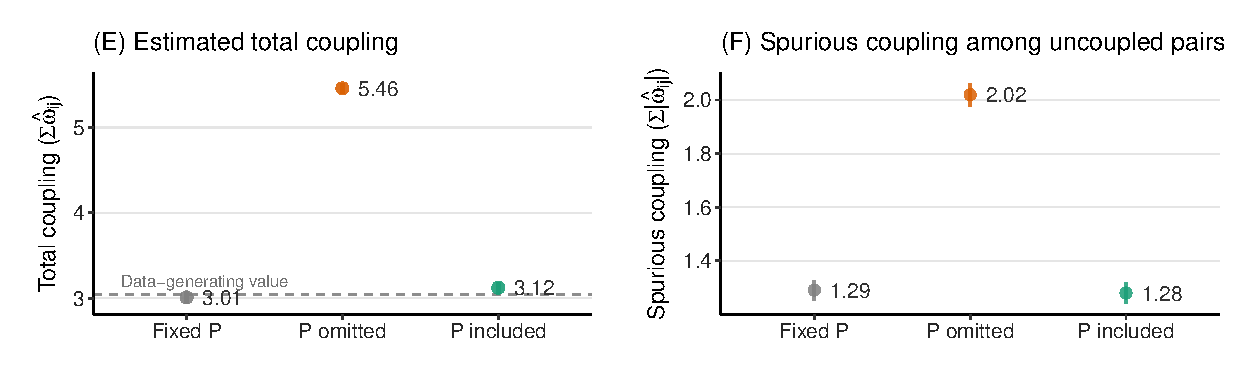
\includegraphics[width=0.82\textwidth]{figs/revision_2026/Figure4_metric_strip.pdf}
\caption{\textbf{Omitting slow context makes estimated symptom networks look more connected.}
(A) True symptom--symptom coupling matrix used to generate the data.
(B) Network estimated from pooled symptom profiles when the slow contextual field varies across people but is omitted from the estimator. Orange edges mark phantom couplings: connections absent in the true network that nonetheless appear in this estimate.
(C) Network estimated from the same pooled data after including the slow contextual field as a covariate.
(D) Omitting \(P\) produces the largest excess estimated global strength relative to the true coupling matrix.
(E) Error on truly absent edges is also largest when \(P\) is omitted, indicating more apparent coupling among symptom pairs with no true direct edge. Points and intervals in panels D--E show means and standard errors across 30 independent replicates.}
\label{fig:network-estimation}
\end{figure}

\section{Discussion}
\subsection{Main contribution}
The main point of the model is simple. A symptom network does not operate in isolation. It is embedded in slower conditions that can make symptoms easier or harder to activate. By putting these pieces in the same model, we can separate
three things that are often blurred together in empirical network comparisons:
symptom-specific activation tendencies, symptom--symptom coupling, and slow
contextual input.

\subsection{Slow context changes activation without changing coupling}
Simulation 1 showed that the same fixed symptom--symptom coupling matrix can
produce different activation distributions depending on the slow contextual
baseline it is embedded in. This is the simplest version of the paper's central
claim: differences in observed symptom activation do not, by themselves, imply
differences in how symptoms are coupled to one another.

\subsection{Feedback can slow recovery}
Simulations 2 and 3 showed that an acute perturbation to the slow field
produces a temporary rise in symptom activation followed by recovery, and that
feedback from sustained symptom activation back into the slow field slows this
recovery. At the moderate feedback strength used in the main recovery
comparison, the system still recovered. Feedback changed the timescale of
recovery, not its eventual outcome.

\subsection{History-dependence under stronger feedback}
Extending the same model across a wider range of feedback strengths showed that
slower recovery is a matter of degree only up to a point. In this parameter
grid, history-dependence emerged around \(b\approx1.0\): trajectories starting
from different initial activation states no longer converged to the same late
state. This is a different regime, not just a slower version of the same
recovery process, in line with critical-transition accounts that emphasize
tipping points and slowed recovery near a transition boundary \parencite{van2014critical, scheffer2009early, helmich2021early}.

This history-dependence emerged from the heterogeneous, symptom-level model
used throughout the paper. It does not rely on the homogeneous mean-field
approximation that motivated earlier versions of the model. We therefore treat
it as a possible regime of the revised model. At the same time, the feedback
strengths at which it appears are stronger than the value used in the main
recovery comparison, and its correspondence to specific clinical phenomena,
such as diagnostic transitions or relapse, remains an open question.

\subsection{When context looks like coupling}
Simulation 4 showed that omitting the slow contextual field from an estimated
symptom network inflated apparent connectivity, including apparent edges
between symptom pairs with no true direct coupling. Including the slow field as
a covariate reduced this inflation. This does not mean that estimated edges are
always artifacts. It means that apparent coupling can partly come from a slower
condition that the model did not include, extending existing equivalence
results between direct-interaction, common-cause, and latent-variable
accounts of symptom association \parencite{kruis2016three, marsman2018introduction, van2021latent} to a setting in which the shared cause is a
dynamic, slowly changing process rather than a static one.

\subsection{Limitations}
Several limitations should temper how these results are interpreted. The
simulations are theoretical and are not calibrated to a specific clinical
population. The slow contextual field is one-dimensional, and symptom states
are binary, both simplifications relative to real symptom measurement.
Symptom--symptom couplings in these examples are positive only. Parameter
choices throughout are illustrative rather than fitted to data. The
context-adjusted estimator used in Simulation 4 corrects for a specific, known
source of contextual variation in this simulation and is not a general causal
identification strategy. Finally, the history-dependent regime identified here
has not been validated against real longitudinal transitions and should not yet
be interpreted as evidence for clinical tipping points.

\subsection{Conclusion}
Fast psychological states do not unfold in isolation from slower contextual
conditions. By embedding a symptom-level network in a slower contextual field,
the present model shows how slow context can shift activation, shape recovery,
prolong persistence through feedback, produce history-dependent regimes under
stronger feedback, and alter the interpretation of estimated symptom networks.
The main implication is not that symptom--symptom coupling is unimportant, but
that coupling and context need to be modeled together when interpreting
psychological dynamics.

\section{Open Practices Statement}
% PLACEHOLDER -- fill in with actual repository URL / OSF link once finalized.
The simulation code, analysis scripts, and figure-generation scripts for this
paper are available at [repository URL to be added]. None of the simulations
reported here involved human participants; all data were computer-generated.
No part of this study was preregistered.

\section{Data Availability Statement}
% PLACEHOLDER -- confirm exact wording matches journal requirements.
All data reported in this paper are simulated. The code used to generate,
analyze, and visualize the simulated data is publicly available at
[repository URL to be added]. No human-subjects data were collected or used.

\section{Author Contributions}
% PLACEHOLDER -- confirm roles against actual contributions (e.g., CRediT taxonomy).
K.P. and V.V.V. conceptualized and developed the computational model. K.P.
implemented the simulations, conducted the analyses, and drafted the
manuscript. D.B., M.L., L.W., J.B., and V.V.V. contributed to conceptual
development and provided critical revisions to the manuscript. All authors
approved the final version for submission.

\section{Conflict of Interest Statement}
% PLACEHOLDER -- confirm with all authors.
The authors declare no conflicts of interest.

\section{Funding}
% PLACEHOLDER -- fill in actual grant/funding source(s), or state no external funding was received.
[Funding source(s) to be added, or a statement that no external funding was received.]

\printbibliography

\end{document}
